\begin{chapter}{Restlessness Extensions}
    \label{chap:extensions}

    % \section{Authentication}
    % auth-jwt and auth-cognito packages

    % \subsection{Usage example}
    % @todo

    \section{Data Access Object}
    \label{sec:data_access_object}

    To simplify the creation of a Data Access Object, Restlessness provides the
    abstract class DaoPackage (listing \ref{lst:daopackage}), which extends the
    AddOnPackage class previously defined.

    \bigskip
    \begin{lstlisting}[caption=DaoPackage class definition, label={lst:daopackage}]
abstract class DaoPackage extends AddOnPackage {
    abstract modelTemplate(modelName: string): string
}
    \end{lstlisting}

    In addition to the previously defined hooks, classes implementing DaoPackage,
    should implement also the modelTemplate method, and a base dao class, to which
    we will refer to as DaoBase. This latter class should provides the main Dao
    functionalities, while the code template returned by modelTemplate should define
    a class that extends the DaoBase one.

    \subsection{Dao for mongodb}
    Restlessness already provides a Dao package for the popular non relational
    database \href{https://www.mongodb.com/}{mongodb}, and it's available on the
    npm platform as \mbox{\textit{@restlessness/dao-mongo}}.
    That package exports two main components, an implementation of the DaoPackage
    class, and a MongoBase class, the base class containing the main Dao
    functionalities for CRUD operations, as shown on listing \ref{fig:mongobase}.

    \begin{figure}
        \centering
        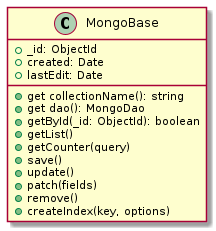
\includegraphics[width=5.5cm]{source/diagrams/mongobase_class.png}
        \caption{MongoBase class}
        \label{fig:mongobase}
    \end{figure}

    Users of the package can then create models based on the MongoBase class through
    the Restlessness Web Interface.
    The creation of that model is made possible by implementing the DaoPackage.modelTemplate
    method, as shown on listing \ref{lst:model_template}.

    \bigskip
    \begin{lstlisting}[caption=modelTemplate function definition, label={lst:model_template}]
const modelTemplate = (name: string): string => `
import {
    MongoBase, ObjectId
} from '@restlessness/dao-mongo';

export default class ${name} extends MongoBase {
    ['constructor']: typeof ${name}

    static get collectionName() {
        return '${pluralize(name, 2).toLowerCase()}';
    }
};
`;
    \end{lstlisting}

    \subsubsection{Database Proxy}
    \label{subsec:database_proxy}
    The MongoBase class uses the MongoDao class internally to perform database
    operations. The latter class, at the early stage of Restlessness development,
    offered an abstraction layer over the official
    \href{https://www.npmjs.com/package/mongodb}{mongodb driver} for Node.js,
    effectively using the driver internally.
    As described on chapter \ref{chap:application}, this approach showed its
    drawbacks in the context of a serverless application, so the next approach has
    been to exploit the concept of Database Proxy.
    The main idea is to have a serverless function, the proxy, with the task of
    performing all database access, on behalf of all other serverless functions.
    Another advantage of Serverless is indeed the possibility to invoke a function
    from another one, but this comes at the cost of a doubled Cold start (
    \ref{subsec:cold_start}), resulting in a performance degradation for some requests.
    However the solution provided on \ref{subsec:cold_start} is particularly useful in
    this case because enabling the warmup plugin on the proxy function, avoids the
    costs of function initialization and also database connection, making it possible
    to enable warmup only on a small group of functions, so the overall performance
    improves or stays the same.

    \begin{figure}
        \centering
        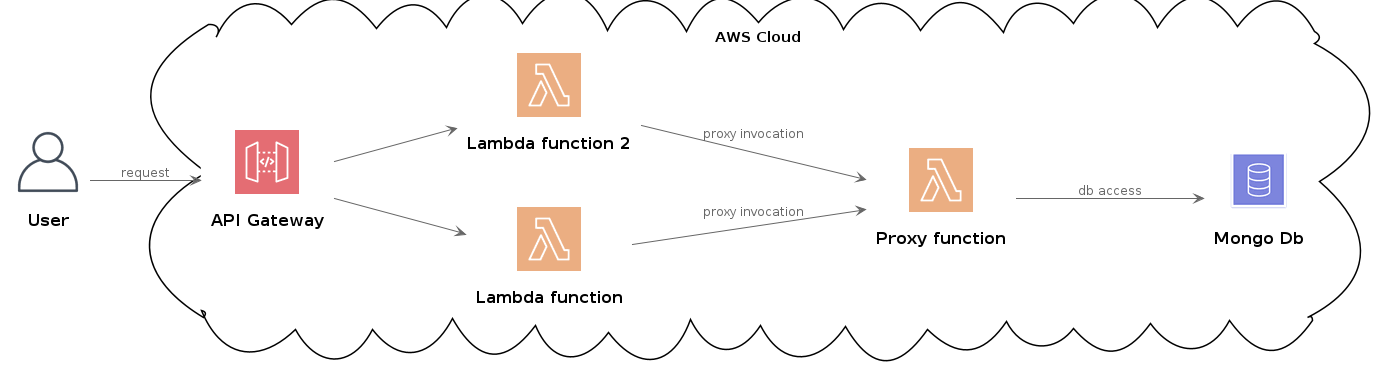
\includegraphics[width=\linewidth]{source/diagrams/mongo_proxy.png}
        \caption{Mongo proxy structure}
    \end{figure}

    To implement this structure has been developed a serverless plugin, named
    \href{https://www.npmjs.com/package/serverless-mongo-proxy}{serverless-mongo-proxy},
    and usable independently of the Restlessness framework.
    The plugin automatically creates the serverless proxy function in the specified
    service, which in the case of Restlessness is the shared one, so all services
    can exploit the advantages of using a proxy.
    Since all information exchanged between serverless functions must be serialized,
    the plugin used the \href{http://bsonspec.org/}{bson} encoding, to obtain consistent
    representation for data types such as dates and regular expressions.

    The MongoDao class can then invoke the proxy function internally, without having
    to keep a connection open.

    \subsection{Usage example}
    The package can be used on a Restlessness project following this steps:

    \paragraph{Installation}
    It is possible to install the package using the npm CLI and then adding it to
    the enabled restlessness addons using the restlessness CLI command add-dao
    (\ref{lst:dao_mongo_install}).

    \bigskip
    \begin{lstlisting}[caption=dao-mongo installation, label={lst:dao_mongo_install}]
$ npm install @restlessness/dao-mongo
$ restlessness add-dao @restlessness/dao-mongo
    \end{lstlisting}

    \paragraph{Model creation}
    Once installed it is possible to create, from the Web Interface, models based on
    the Dao class provided by the package (\ref{fig:wi_dao_mongo_model}).

    This corresponds to the creation of a model template that can be extended with
    methods and fields (\ref{lst:new_model})

    \bigskip
    \begin{lstlisting}[caption=A new model based on the dao-mongo package, label={lst:new_model}]
export default class User extends MongoBase {
  ['constructor']: typeof User
  name: string
  age: number

  static get collectionName() {
    return 'users';
  }
};
    \end{lstlisting}

    \paragraph{Model usage}
    It's then possible to perform database operations, exploiting the abstraction
    provided by the MongoBase class, as shown on \ref{lst:user_model_usage}.

    \bigskip
    \begin{lstlisting}[caption=User model usage, label={lst:user_model_usage}]
const user = new User();
user.name = 'Andrea';
user.age = 25;
await user.save();
    \end{lstlisting}

    \begin{figure}
        \centering
        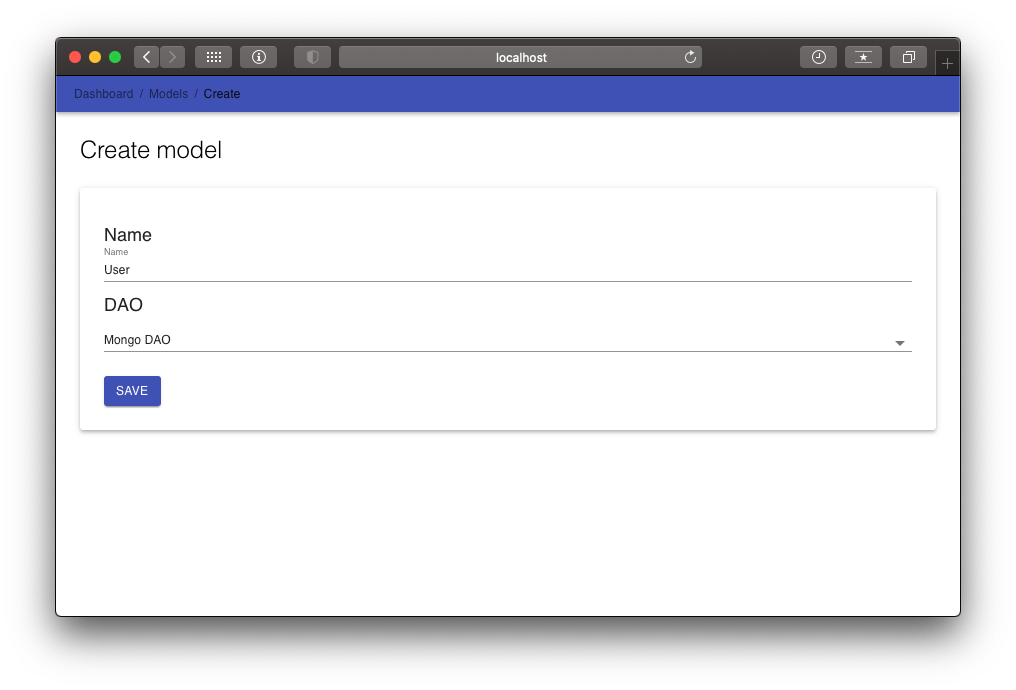
\includegraphics[width=\linewidth]{source/images/rln-wi-create-model.png}
        \caption{Creation of a Model}
        \label{fig:wi_dao_mongo_model}
    \end{figure}

\end{chapter}